\documentclass{article}

\usepackage{fancyhdr}
\usepackage{extramarks}
\usepackage{amsmath}
\usepackage{amsthm}
\usepackage{amsfonts}
\usepackage{tikz}
\usepackage[plain]{algorithm}
\usepackage{algpseudocode}
\usepackage{enumerate}
\usepackage{amsmath}
\usepackage{amssymb}
\usetikzlibrary{automata,positioning}

%
% Basic Document Settings
%

\topmargin=-0.45in
\evensidemargin=0in
\oddsidemargin=0in
\textwidth=6.5in
\textheight=9.0in
\headsep=0.25in

\linespread{1.1}

\pagestyle{fancy}
\lhead{\hmwkAuthorName}
\chead{\hmwkClass\ (\hmwkClassInstructor\ \hmwkClassTime): \hmwkTitle}
\rhead{\firstxmark}
\lfoot{\lastxmark}
\cfoot{\thepage}

\renewcommand\headrulewidth{0.4pt}
\renewcommand\footrulewidth{0.4pt}

\setlength\parindent{0pt}

%
% Create Problem Sections
%

\newcommand{\enterProblemHeader}[1]{
    \nobreak\extramarks{}{Problem \arabic{#1} continued on next page\ldots}\nobreak{}
    \nobreak\extramarks{Problem \arabic{#1} (continued)}{Problem \arabic{#1} continued on next page\ldots}\nobreak{}
}

\newcommand{\exitProblemHeader}[1]{
    \nobreak\extramarks{Problem \arabic{#1} (continued)}{Problem \arabic{#1} continued on next page\ldots}\nobreak{}
    \stepcounter{#1}
    \nobreak\extramarks{Problem \arabic{#1}}{}\nobreak{}
}

\setcounter{secnumdepth}{0}
\newcounter{partCounter}
\newcounter{homeworkProblemCounter}
\setcounter{homeworkProblemCounter}{1}
\nobreak\extramarks{Problem \arabic{homeworkProblemCounter}}{}\nobreak{}

%
% Homework Problem Environment
%
% This environment takes an optional argument. When given, it will adjust the
% problem counter. This is useful for when the problems given for your
% assignment aren't sequential. See the last 3 problems of this template for an
% example.
%
\newenvironment{homeworkProblem}[1][-1]{
    \ifnum#1>0
        \setcounter{homeworkProblemCounter}{#1}
    \fi
    \section{Problem \arabic{homeworkProblemCounter}}
    \setcounter{partCounter}{1}
    \enterProblemHeader{homeworkProblemCounter}
}{
    \exitProblemHeader{homeworkProblemCounter}
}

%
% Homework Details
%   - Title
%   - Due date
%   - Class
%   - Section/Time
%   - Instructor
%   - Author
%

\newcommand{\hmwkTitle}{Tutorial Week 7}
\newcommand{\hmwkDueDate}{February 25, 2021}
\newcommand{\hmwkClass}{CZ4041}
\newcommand{\hmwkClassTime}{CS4}
\newcommand{\hmwkClassInstructor}{Assoc Prof Pan, Sinno Jialin}
\newcommand{\hmwkAuthorName}{\textbf{Pang Yu Shao}}
\newcommand{\hmwkAuthorID}{\textbf{U1721680D}}

%
% Title Page
%

\title{
    \vspace{2in}
    \textmd{\textbf{\hmwkClass:\ \hmwkTitle}}\\
    \normalsize\vspace{0.1in}\small{Due\ on\ \hmwkDueDate\ at 8:30am}\\
    \vspace{0.1in}\large{\textit{\hmwkClassInstructor\ - \hmwkClassTime}}
    \vspace{3in}\\
    \hmwkAuthorName\\
    \hmwkAuthorID
}

\date{25/02/2021}

\renewcommand{\part}[1]{\textbf{\large Part \Alph{partCounter}}\stepcounter{partCounter}\\}

%
% Various Helper Commands
%

% Useful for algorithms
\newcommand{\alg}[1]{\textsc{\bfseries \footnotesize #1}}

% For derivatives
\newcommand{\deriv}[1]{\frac{\mathrm{d}}{\mathrm{d}x} (#1)}

% For partial derivatives
\newcommand{\pderiv}[2]{\frac{\partial}{\partial #1} (#2)}

% Integral dx
\newcommand{\dx}{\mathrm{d}x}

% Alias for the Solution section header
\newcommand{\solution}{\textbf{\large Solution}}

% Probability commands: Expectation, Variance, Covariance, Bias
\newcommand{\E}{\mathrm{E}}
\newcommand{\Var}{\mathrm{Var}}
\newcommand{\Cov}{\mathrm{Cov}}
\newcommand{\Bias}{\mathrm{Bias}}

\begin{document}

\maketitle

\pagebreak

\begin{homeworkProblem}
    On the 21th page of the lecture notes "Lecture 7b", we have shown how
    to use backpropagation to update parameter of the ANN with one initialization setting
    for w. Suppose now we initialize w with another set of values: w13 = -1, w14 = -1,
    w23 = -1, w24 = -1, w35 = -1, and w45 = -1. Run one epoch (i.e., run through the
    whole training dataset once), to show how the parameters are updated at each iteration.
    \\\\

    \textbf{Solution}\\
    Training Record: (0,0,-1)
    Forward pass:
    \[
        \begin{split}
        h_1 &= 0\\
        h_2 &= 0\\
        h_3 &= sign(0*-1 + 0*-1) = 1\\
        h_4 &= sign(0*-1 + 0*-1) = 1\\
        h_5 &= sign(1*-1 + 1*-1) = -1\\
        \end{split}
    \]
    No weights updated.\\
    Training Record: (1,0,1)
    Forward pass:
    \[
        \begin{split}
        h_1 &= 1\\
        h_2 &= 0\\
        h_3 &= sign(1*-1 + 0*-1) = -1\\
        h_4 &= sign(1*-1 + 0*-1) = -1\\
        h_5 &= sign(-1*-1 + -1*-1) = 1\\
        \end{split}
    \]
    No weights updated.\\
    Training Record: (0,1,1)
    Forward pass:
    \[
        \begin{split}
        h_1 &= 0\\
        h_2 &= 1\\
        h_3 &= sign(0*-1 + 1*-1) = -1\\
        h_4 &= sign(0*-1 + 1*-1) = -1\\
        h_5 &= sign(-1*-1 + -1*-1) = 1\\
        \end{split}
    \]
    No weights updated.\\
    Training Record: (1,1,1)
    Forward pass:
    \[
        \begin{split}
        h_1 &= 1\\
        h_2 &= 1\\
        h_3 &= sign(1*-1 + 1*-1) = -1\\
        h_4 &= sign(1*-1 + 1*-1) = -1\\
        h_5 &= sign(-1*-1 + -1*-1) = 1\\
        \end{split}
    \]
    No weights updated.\\
    \textbf{End of epoch 1}
\end{homeworkProblem}
\newpage
\begin{homeworkProblem}
    Consider a 2-dimensional dataset for three-class classification by ANN,
    as shown in Figure 1. Which ANN model as shown in Figure 2 is proper to solve the classification
    problem? and why?

    \begin{figure}[H]
        \begin{center}
        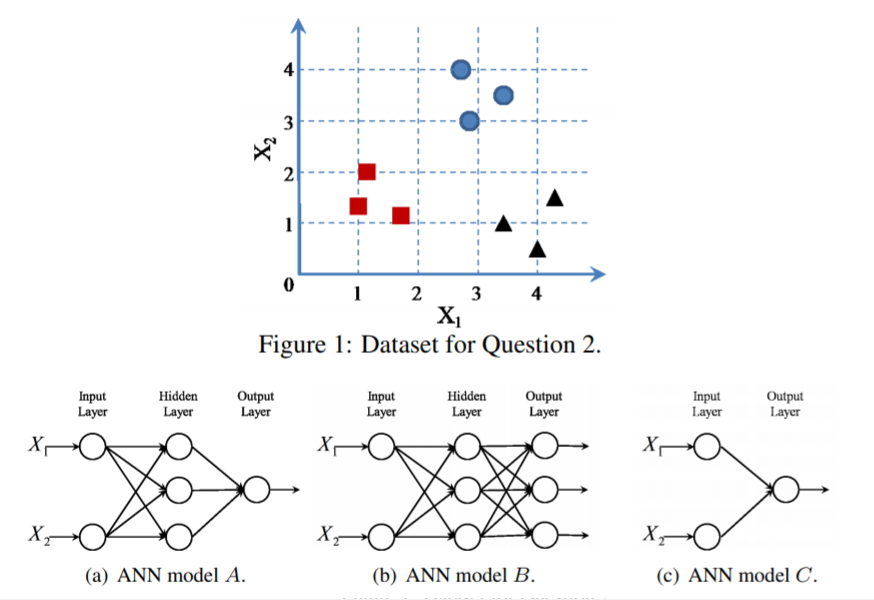
\includegraphics{resources/q2.PNG}
        \end{center}
    \end{figure}

    \textbf{Solution}\\
    \textbf{ANN model B} is the proper model to be used as it has 3 output neurons, which is the 
    proper implementation for a three-class classification problem. The output would be probabilities
    (or prediction) of the input features and the output having the highest value (i.e, highest Probability)
    would be chosen as the predicted label. 
\end{homeworkProblem}

\newpage
\begin{homeworkProblem}
    Compute the derivative of the sigmoid function $f(z) = \frac{1}{1+e^{-z}}$ w.r.t z.
    \\\\
    \textbf{Solution}\\
    Let $u = 1 + e^{-z}$\\
    \[
        \begin{split}
        f(u) &= 1/u\\
        f'(u) &= -1/u^2\\\\
        \frac{du}{dz} &= -e^{-z}\\\\
        \therefore f'(z) &= f'(u)*\frac{du}{dz}\\
        &= \frac{e^{-z}}{u^2}\\
        &= \frac{e^{-z}}{(1 + e^{-z})^2}\\
        &= \frac{1}{1 + e^{-z}}(\frac{e^{-z}}{1 + e^{-z}})\\
        &= f(z)(1 - \frac{1}{1 + e^{-z}})\\
        &= f(z)(1 - f(z))
        \end{split}
    \]
\end{homeworkProblem}
\end{document}